
% plantilla obtenida de: https://www.overleaf.com/19886281jjqffwsxshmm#/73112823/

\documentclass[a4paper, 11pt]{article}
\usepackage{comment} % enables the use of multi-line comments (\ifx \fi) 
\usepackage{lipsum} %This package just generates Lorem Ipsum filler text. 
\usepackage{fullpage} % changes the margin

\usepackage[spanish]{babel}
\usepackage[utf8]{inputenc}

\usepackage{graphicx}

\usepackage{amsmath}
\usepackage{amsfonts}
% or
\usepackage{amssymb}
\usepackage{tikz}
\usepackage{array}
\newcolumntype{C}{>{$}l<{$}} % math-mode version of "l" column type
\newcommand{\imageins}[4]{\begin{figure}[!ht]		%Take the hardwork from using images. Let this command do the work for you. Insert images by just using this command \imageins{filename}{width as a ratio of total text width of the page}{caption name}{label name for referring in articles}		
    \centering
    \includegraphics[width=#2\textwidth]{#1}
    %\caption{#3}
    %\label{#4}
    \vspace{0.2em}
\end{figure}}

%%%%%%%%%%%%%%%%%%%%%%%%%%%%%%%%%%%%%%%%%%%%%%%%%%%%%%%%%%%%%%%%%%%%%%%%%%%%%%%%%%
\usepackage{listings}
\usepackage{color}
 
\definecolor{codegreen}{rgb}{0,0.6,0}
\definecolor{codegray}{rgb}{0.5,0.5,0.5}
\definecolor{codepurple}{rgb}{0.58,0,0.82}
\definecolor{backcolour}{rgb}{0.95,0.95,0.92}
 
\lstdefinestyle{mystyle}{
    backgroundcolor=\color{backcolour},   
    commentstyle=\color{codegreen},
    keywordstyle=\color{magenta},
    numberstyle=\tiny\color{codegray},
    stringstyle=\color{codepurple},
    basicstyle=\footnotesize,
    breakatwhitespace=false,         
    breaklines=true,                 
    captionpos=b,                    
    keepspaces=true,                 
    numbers=left,                    
    numbersep=5pt,                  
    showspaces=false,                
    showstringspaces=false,
    showtabs=false,                  
    tabsize=2
}
 
\lstset{style=mystyle}

%%%%%%%%%%%%%%%%%%%%%%%%%%%%%%%%%%%%%%%%%%%%%%%%%%%%%%%%%%%%%%%%%%%%%%%%%%%%%%%%%%

\begin{document}
%Header-Make sure you update this information!!!!
\noindent
\large\textbf{Relación III} \hfill \textbf{Antonio Gámiz Delgado} \\
\normalsize Modelos de Computación \hfill 6/11/2018
%\normalsize ECE 100-003 \hfill Teammates: Student1, Student2 \\
%Prof. Oruklu \hfill Lab Date: XX/XX/XX \\
%TA: Adam Sumner \hfill Due Date: XX/XX/XX

\section*{Ejercicio 27}
Construir expresiones regulares para los siguientes lenguajes sobre el alfabeto $\{0,1\}$:
\begin{enumerate}
\item Palabras en las que el número de símbolos 0 es múltiplo de 3.
\[
(1^*01^*01^*01^*)^*
\]
\item Palabras que contienen como subcadena a 1100 ó a 00110.
\[
(0+1)^*(1100+00110)(0+1)^*
\]
\item Palabras en las que cada cero forma parte de una subcadena de 2 ceros y cada 1 forma parte de una subcadena de 3 unos.
\[
(00^++111^+)^*
\]
\item Palabras en las que el número de ocurrencias de la subcadena 011 es menor o igual que el de ocurrencias de la subcadena 110.

Este lenguaje no es regular, por lo que no tiene expresión regular asociada. Usemos el lema de Bombeo para demostrarlo: $L=\{\text{ lenguaje del enunciado }\}$.
El lema de Bombeo dice que:

Si $L$ es un conjunto regular, entonces existe unu $n\in\mathbb{N}$ tal que $\forall z \in L$, si $|z|\geq n$, entonces $z$ se puede expresar de la forma $z=uvw$, donde:
\begin{itemize}
\item $|uv|\leq n$
\item $|v|\geq 1$
\item $(\forall i \geq 0) \enskip uv^iw \in L$
\end{itemize}

Por lo que tomando $z = (011)^n(110)^n\in L$ y como descomposición $u=\varepsilon$, $v=(011)^n$ y $w=(110)^n$ y $i=2$, entonces:
\[
uv^iw=v^iw=(011)^{2n}(110)^n\notin L \enskip \forall n \in \mathbb{N}
\]

Luego $L$ no es regular.

\end{enumerate}

\section*{Ejercicio 29}
Encuentra para cada uno de los siguientes lenguajes una gramática de tipo 3 que lo genere o un autómata finito que lo reconozca.
\begin{itemize}
\item $L_1=\{ u\in\{0,1\}^*:\enskip u \text{ no contiene la subcadena '0101' } \}$

\begin{center}
\begin{tikzpicture}[scale=0.2]
\tikzstyle{every node}+=[inner sep=0pt]
\draw [black] (13.8,-19.9) circle (3);
\draw (13.8,-19.9) node {$q_0$};
\draw [black] (13.8,-19.9) circle (2.4);
\draw [black] (29,-19.9) circle (3);
\draw (29,-19.9) node {$q_1$};
\draw [black] (29,-19.9) circle (2.4);
\draw [black] (42,-20) circle (3);
\draw (42,-20) node {$q_2$};
\draw [black] (42,-20) circle (2.4);
\draw [black] (55.1,-19.9) circle (3);
\draw (55.1,-19.9) node {$q_3$};
\draw [black] (55.1,-19.9) circle (2.4);
\draw [black] (68,-19.9) circle (3);
\draw (68,-19.9) node {$\varnothing$};
\draw [black] (12.477,-17.22) arc (234:-54:2.25);
\draw (13.8,-12.65) node [above] {$1$};
\fill [black] (15.12,-17.22) -- (16,-16.87) -- (15.19,-16.28);
\draw [black] (66.677,-17.22) arc (234:-54:2.25);
\draw (68,-12.65) node [above] {$1,0$};
\fill [black] (69.32,-17.22) -- (70.2,-16.87) -- (69.39,-16.28);
\draw [black] (27.677,-17.22) arc (234:-54:2.25);
\draw (29,-12.65) node [above] {$0$};
\fill [black] (30.32,-17.22) -- (31.2,-16.87) -- (30.39,-16.28);
\draw [black] (16.8,-19.9) -- (26,-19.9);
\fill [black] (26,-19.9) -- (25.2,-19.4) -- (25.2,-20.4);
\draw (21.4,-20.4) node [below] {$0$};
\draw [black] (32,-19.92) -- (39,-19.98);
\fill [black] (39,-19.98) -- (38.2,-19.47) -- (38.2,-20.47);
\draw (35.5,-20.46) node [below] {$1$};
\draw [black] (45,-19.98) -- (52.1,-19.92);
\fill [black] (52.1,-19.92) -- (51.3,-19.43) -- (51.3,-20.43);
\draw (48.55,-20.46) node [below] {$0$};
\draw [black] (58.1,-19.9) -- (65,-19.9);
\fill [black] (65,-19.9) -- (64.2,-19.4) -- (64.2,-20.4);
\draw (61.55,-20.4) node [below] {$1$};
\draw [black] (41.145,-22.87) arc (-22.5812:-157.82515:14.335);
\fill [black] (14.63,-22.78) -- (14.47,-23.71) -- (15.4,-23.33);
\draw (27.86,-32.2) node [below] {$1$};
\draw [black] (54.614,-22.854) arc (-15.92751:-164.07249:13.065);
\fill [black] (29.49,-22.85) -- (29.23,-23.76) -- (30.19,-23.49);
\draw (42.05,-32.83) node [below] {$0$};
\draw [black] (10,-19.9) -- (10.8,-19.9);
\fill [black] (10.8,-19.9) -- (10,-19.4) -- (10,-20.4);
\end{tikzpicture}
\end{center}

\item $L_1=\{ 0^i1^j0^k:\enskip i\geq 1, \enskip k \geq 0, i \text{ impar}, k \text{ múltiplo de 3}, j\geq 2 \}$

\begin{center}
\begin{tikzpicture}[scale=0.2]
\tikzstyle{every node}+=[inner sep=0pt]
\draw [black] (13.2,-13.8) circle (3);
\draw (13.2,-13.8) node {$q_0$};
\draw [black] (26.5,-13.8) circle (3);
\draw (26.5,-13.8) node {$q_1$};
\draw [black] (40.2,-13.8) circle (3);
\draw (40.2,-13.8) node {$q_2$};
\draw [black] (53.2,-13.8) circle (3);
\draw (53.2,-13.8) node {$q_3$};
\draw [black] (53.2,-13.8) circle (2.4);
\draw [black] (26.5,-27.9) circle (3);
\draw (26.5,-27.9) node {$q_9$};
\draw [black] (11.1,-38) circle (3);
\draw (11.1,-38) node {$q_6$};
\draw [black] (11.1,-38) circle (2.4);
\draw [black] (26.5,-38) circle (3);
\draw (26.5,-38) node {$q_4$};
\draw [black] (41.9,-38) circle (3);
\draw (41.9,-38) node {$q_5$};
\draw [black] (9.8,-13.8) -- (10.2,-13.8);
\fill [black] (10.2,-13.8) -- (9.4,-13.3) -- (9.4,-14.3);
\draw [black] (15.943,-12.601) arc (107.13018:72.86982:13.264);
\fill [black] (23.76,-12.6) -- (23.14,-11.89) -- (22.85,-12.84);
\draw (19.85,-11.51) node [above] {$0$};
\draw [black] (23.821,-15.134) arc (-70.6877:-109.3123:12.009);
\fill [black] (15.88,-15.13) -- (16.47,-15.87) -- (16.8,-14.93);
\draw (19.85,-16.31) node [below] {$0$};
\draw [black] (29.5,-13.8) -- (37.2,-13.8);
\fill [black] (37.2,-13.8) -- (36.4,-13.3) -- (36.4,-14.3);
\draw (33.35,-14.3) node [below] {$1$};
\draw [black] (43.2,-13.8) -- (50.2,-13.8);
\fill [black] (50.2,-13.8) -- (49.4,-13.3) -- (49.4,-14.3);
\draw (46.7,-14.3) node [below] {$1$};
\draw [black] (51.877,-11.12) arc (234:-54:2.25);
\draw (53.2,-6.55) node [above] {$1$};
\fill [black] (54.52,-11.12) -- (55.4,-10.77) -- (54.59,-10.18);
\draw [black] (23.757,-26.691) arc (-117.80661:-155.53818:21.431);
\fill [black] (23.76,-26.69) -- (23.28,-25.88) -- (22.82,-26.76);
\draw (17.63,-23.91) node [left] {$1$};
\draw [black] (39.379,-16.682) arc (-20.66561:-67.68571:18.026);
\fill [black] (29.36,-27) -- (30.29,-27.16) -- (29.91,-26.23);
\draw (35.97,-24.35) node [right] {$0$};
\draw [black] (25.177,-25.22) arc (234:-54:2.25);
\draw (26.5,-20.65) node [above] {$0,1$};
\fill [black] (27.82,-25.22) -- (28.7,-24.87) -- (27.89,-24.28);
\draw [black] (14.1,-38) -- (23.5,-38);
\fill [black] (23.5,-38) -- (22.7,-37.5) -- (22.7,-38.5);
\draw (18.8,-38.5) node [below] {$0$};
\draw [black] (29.5,-38) -- (38.9,-38);
\fill [black] (38.9,-38) -- (38.1,-37.5) -- (38.1,-38.5);
\draw (34.2,-38.5) node [below] {$0$};
\draw [black] (39.591,-39.912) arc (-54.21866:-125.78134:22.389);
\fill [black] (13.41,-39.91) -- (13.77,-40.79) -- (14.35,-39.97);
\draw (26.5,-44.64) node [below] {$o$};
\draw [black] (13.61,-36.35) -- (23.99,-29.55);
\fill [black] (23.99,-29.55) -- (23.05,-29.57) -- (23.6,-30.4);
\draw (17.8,-32.45) node [above] {$1$};
\draw [black] (26.5,-35) -- (26.5,-30.9);
\fill [black] (26.5,-30.9) -- (26,-31.7) -- (27,-31.7);
\draw (27,-32.95) node [right] {$1$};
\draw [black] (39.39,-36.35) -- (29.01,-29.55);
\fill [black] (29.01,-29.55) -- (29.4,-30.4) -- (29.95,-29.57);
\draw (35.2,-32.45) node [above] {$1$};
\draw [black] (51.963,-16.532) arc (-26.42004:-69.20371:41.854);
\fill [black] (29.34,-37.04) -- (30.27,-37.22) -- (29.91,-36.28);
\draw (43.6,-29.41) node [below] {$0$};
\end{tikzpicture}
\end{center}

\end{itemize}

Como $L_2\subset L_1 \Longrightarrow L_2 = L_1\cup L_2$, luego el segundo autómata finito determinista es también el AFD de la intersección.

\section*{Ejercicio 45}
Sea el alfabeto $A=\{0,1,+,=\}$, demostrar que el lenguaje
\[
ADD=\{x=y+z|x,y,z \text{ son números en binario, y x es la suma de y y z}\}
\]
no es regular.

Usando el lema de Bombeo enunciado anteriormente, tenemos que cogiendo $z=1^n+0=1^n\in ADD$, $u=\varepsilon$, $v=1^n$ y $w=+0=1^n$ y $i=2$:
\[
uv^iw=v^iw=1^{2n}+0=1^n \notin ADD \enskip \forall n \in \mathbb{N}
\]

Por lo tanto, ADD no es regular.

\section*{Ejercicio 46}
Si $L_1,L_2$ son lenguajes sobre el alfabeto $A$, entonces la \textit{mezcla perfecta} de estos lenguajes se define como el lenguaje:
\[
\{w|w=a_1b_1...a_kb_k \enskip \text{ donde } a_1...a_k\in L_1, \enskip b_1...b_k\in L_2, \enskip a_i, b_i \in A\}
\]

Demostrar que si $L_1$ y $L_2$ son regulares, entonces la mezcla perfecta de $L_1$ y $L_2$ es regular.

No sé hacerlo :(.

\section*{Ejercicio 47}
Minimizar el autómata:
\begin{center}
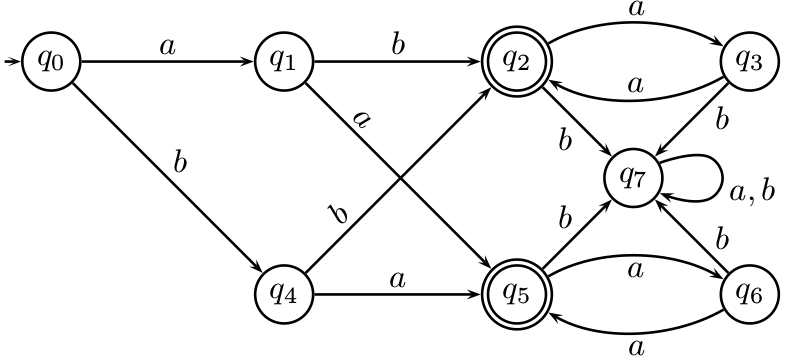
\includegraphics[scale=0.5]{ejercicio47.png}
\end{center}

Podemos ver que $q_1 \equiv q_4$, $q_2 \equiv q_5$ y $q_3 \equiv q_6$. Luego nos quedaría:

\begin{center}
\begin{tikzpicture}[scale=0.2]
\tikzstyle{every node}+=[inner sep=0pt]
\draw [black] (10.6,-28.2) circle (3);
\draw (10.6,-28.2) node {$q_0$};
\draw [black] (24.3,-28.2) circle (3);
\draw (24.3,-28.2) node {$q_1$};
\draw [black] (37.6,-28.2) circle (3);
\draw (37.6,-28.2) node {$q_2$};
\draw [black] (37.6,-28.2) circle (2.4);
\draw [black] (49.6,-28.2) circle (3);
\draw (49.6,-28.2) node {$q_3$};
\draw [black] (63.1,-28.2) circle (3);
\draw (63.1,-28.2) node {$q_7$};
\draw [black] (13.6,-28.2) -- (21.3,-28.2);
\fill [black] (21.3,-28.2) -- (20.5,-27.7) -- (20.5,-28.7);
\draw (17.45,-27.7) node [above] {$a,b$};
\draw [black] (6.9,-28.2) -- (7.6,-28.2);
\fill [black] (7.6,-28.2) -- (6.8,-27.7) -- (6.8,-28.7);
\draw [black] (27.3,-28.2) -- (34.6,-28.2);
\fill [black] (34.6,-28.2) -- (33.8,-27.7) -- (33.8,-28.7);
\draw (30.95,-27.7) node [above] {$a,b$};
\draw [black] (40.124,-26.604) arc (112.73965:67.26035:8.992);
\fill [black] (40.12,-26.6) -- (41.06,-26.76) -- (40.67,-25.83);
\draw (43.6,-25.41) node [above] {$a$};
\draw [black] (47.166,-29.927) arc (-64.87563:-115.12437:8.399);
\fill [black] (47.17,-29.93) -- (46.23,-29.81) -- (46.65,-30.72);
\draw (43.6,-31.22) node [below] {$a$};
\draw [black] (52.6,-28.2) -- (60.1,-28.2);
\fill [black] (60.1,-28.2) -- (59.3,-27.7) -- (59.3,-28.7);
\draw (56.35,-27.7) node [above] {$b$};
\draw [black] (63.686,-25.27) arc (196.43141:-91.56859:2.25);
\draw (68.91,-22.35) node [above] {$a,b$};
\fill [black] (65.78,-26.88) -- (66.69,-27.14) -- (66.41,-26.18);
\draw [black] (39.72,-26.083) arc (129.7894:50.2106:16.611);
\fill [black] (60.98,-26.08) -- (60.69,-25.19) -- (60.05,-25.96);
\draw (50.35,-21.74) node [above] {$b$};
\end{tikzpicture}
\end{center}
 

\end{document}